\subsection*{Test of CAN and queues} \label{sec:test_of_queues}
In order to test CAN and queues, a task was written. The purpose of the task was to receive a CAN-message if any available from the queue and send the ID and data from the CAN message to a PC using UART.
The task used can be seen in code \ref{code:test_can_uart_task}.


\begin{lstlisting}[language = c, caption = Snippet of task used to test CAN, label=code:test_can_uart_task]
CAN_frame frame;
if(QueueReceive(&Queue_CAN_Rx, &frame)) {
	char ch;
	/* ID out uart0 */
	for(int i = 3; i >=0; i--){
		ch = ((frame.id >> i*8) & 0x000000FF);
		QueueSend(&Queue_Uart0_Tx,&ch);
	}
	/* ID end*/

	/* MSG out uart0 */
	for(int i = (frame.dlc-1); i >=0; i--){
		ch = ((frame.msg >> i*8) & 0x00000000000000FF);
		QueueSend(&Queue_Uart0_Tx,&ch);
	}
	/* MSG end */

	/* End of line */
	ch = '\r';
	QueueSend(&Queue_Uart0_Tx,&ch);
	ch = '\n';
	QueueSend(&Queue_Uart0_Tx,&ch);
}
\end{lstlisting}
The command used to send CAN-messages can be seen in code \ref{code:bash_send_can}.

\begin{lstlisting}[language = bash, caption = Task used to test CAN, label=code:bash_send_can]
while true; do sleep 1; print $(date); cansend can0  1DEADBEF#FEDCBA9876543210; done
\end{lstlisting}
The command sends a CAN-message using a connected PEAK-CAN adapter. It sends a message each second and prints out the date to make it clear when it is sending a message.\\ \textit{1deadbef} is the 29 bit ID and \textit{fedcba9876543210} is the 64 bit data. \\


The command used to show the received HEX values can be seen in code \ref{code:xxd}

\begin{lstlisting}[language = bash, caption = Command used to get UART messages, label=code:xxd]
cat /dev/ttyUSB0 | xxd -c 14 
\end{lstlisting}
Cat reads from /dev/ttyUSB0 and pipes its output to xxd where it is shown in HEX.\\ -c is number of columns which is 14 due to 4 ID bytes, 8 data bytes and 2 as newline.\\

The result can be seen in figure \ref{fig:can_recv_output}.
\begin{figure}[H]
    \center
    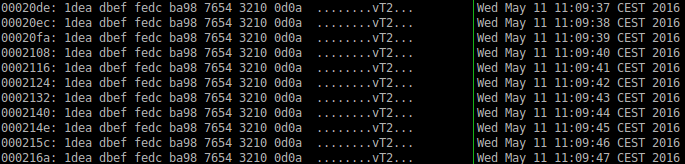
\includegraphics[width=1\textwidth]{graphics/xdd_can_test.png}
  \label{fig:boat1}
  \caption{Left shows output from command \ref{code:xxd} and right shows command \ref{code:bash_send_can}}
\end{figure}
It can be seen that the received ID and data is \textit{1deadbef} and \textit{fedcba9876543210} respectively.\\
\textit{0d0a} is \textbackslash r and \textbackslash n respectively.


